\documentclass[11pt,a4paper]{article}
\usepackage{fontspec}
\usepackage{xeCJK}
\setCJKmainfont{STSong}
\setCJKsansfont{STHeiti}
\usepackage{amsmath,amssymb,amsthm}
\usepackage{mathtools}
\usepackage{bm}
\usepackage{booktabs}
\usepackage{array}
\usepackage{enumitem}
\usepackage{geometry}
\usepackage{xcolor}
\usepackage{tcolorbox}
\usepackage{algorithm}
\usepackage{algpseudocode}
\usepackage{pifont}
\usepackage{graphicx}
\usepackage{subcaption}
\usepackage{tikz}
\usetikzlibrary{arrows.meta,positioning,calc,fit,decorations.pathreplacing}
\usepackage[pdfencoding=auto,psdextra]{hyperref}

\geometry{margin=2.5cm}

\newcommand{\loss}{\mathcal{L}}
\newcommand{\E}{\mathbb{E}}
\newcommand{\R}{\mathbb{R}}
\newcommand{\KL}{\mathrm{KL}}
\newcommand{\N}{\mathcal{N}}
\newcommand{\adv}{\mathcal{A}}
\newcommand{\reward}{R}
\newcommand{\softmax}{\mathrm{softmax}}
\newcommand{\sg}{\mathrm{sg}}
\newcommand{\MoF}{\mathrm{MoF}}
\newcommand{\dom}{\mathrm{dom}}
\newcommand{\OOD}{\mathrm{OOD}}
\newcommand{\const}{\mathrm{const}}
\newcommand{\OPD}{\mathrm{OPD}}
\newcommand{\base}{\mathrm{base}}
\newcommand{\stu}{\theta}

\theoremstyle{definition}
\newtheorem{definition}{定义}
\newtheorem{remark}{注}
\newtheorem{proposition}{命题}
\newtheorem{corollary}{推论}
\newtheorem{lemma}{引理}
\newtheorem{theorem}{定理}
\newtheorem{example}{例}

\title{\textbf{多-Teacher 合并的形式化与``更好混合''判据路线图}\\[0.3em]
\large 从 DiffusionOPD 的平凡路由到凸包约束下的最优混合}
\author{Jayce-Ping}
\date{}

\begin{document}
\maketitle

\begin{abstract}
本文把``将 $K$ 个在不同 prompt set 上、由 single-reward RL 各自训练的 teacher flow model
合并为单个 student''形式化为在 \emph{multi-teacher 路由凸组合}
$v^\stu=\sum_k\lambda_k(t,c)\,v^{(k)}$ 上的优化问题，并理顺``如何得到更好的混合''这一思路。
\textbf{(i)} 在该形式化下，先前工作 DiffusionOPD 的 per-step KL 蒸馏，其最优解恰是一个
\emph{平凡路由}——单 teacher 监督时为 one-hot、多 teacher 监督时为各 teacher velocity 的
监督权重加权均值。\textbf{(ii)} 平凡解继承 single-reward teacher 的
reward-hacking，导致 in-domain 输出分布\emph{坍缩/锐化}，而 prompt-rewriting 只能缓解、不能根治坍缩。
\textbf{(iii)} 由于混合本身即合法 flow model，``更好的混合''可统一写成凸包约束优化
$\max_\lambda Q(v_\lambda)$，真正的难点在于\emph{如何定义} $Q$。我们逐条分析五条候选目标
（旧 / 强 reward RL、training-free user study、min-KL-to-pretrained、真实数据 SFT），并指出
reward 自循环下``更高分 $\neq$ 更好''这一根本困难。本文为 roadmap 文档，凸组合合法性的
自包含证明见附录。
\end{abstract}

\tableofcontents
\newpage

%% ============================================================
\section{引言与问题形式化}
\label{sec:intro}
%% ============================================================

\subsection{动机：从单 reward 专家到统一 student}

现代文生图扩散/流匹配模型的对齐已成为多目标问题：组合准确性（GenEval）、
文字渲染（OCR）、人类偏好（PickScore / Aesthetic）各有其 reward 与训练集。
主流做法是\emph{分而治之}：对每个目标用 single-reward RL 训练一个\emph{专家}
teacher，得到一组互不相同的 LoRA 快照 $\{v^{(k)}\}_{k=1}^K$。但部署需要\emph{单个}
模型同时具备这些能力，于是产生本文的核心问题：

\begin{tcolorbox}[colback=blue!5,colframe=blue!50!black,title=\textbf{核心问题}]
给定 $K$ 个分别在 prompt set $\{\mathcal{P}_k\}$ 上训练好的、冻结的 teacher flow
model $\{v^{(k)}\}$，如何把它们\emph{合并}成单个 student flow model $v^\stu$，使其
在每个 in-domain set 上不退化于对应 teacher，并在 out-of-domain（OOD）prompt 上获得
跨目标的能力增益？或者说，让student flow model获得何种程度的能力提升？
\end{tcolorbox}

\subsection{记号}
\label{ssec:notation}

\begin{center}
\renewcommand{\arraystretch}{1.25}
\footnotesize
\begin{tabular}{@{}l@{\quad}p{11cm}@{}}
\toprule
\textbf{符号} & \textbf{含义} \\
\midrule
$K,\ k$ & teacher 数量与索引 \\
$S,\ s$ & prompt set（source）数量与索引；$s(c)$ = prompt $c$ 的 source \\
$\mathcal{P}_s$ & source $s$ 的 prompt set；$\pi_s=\Pr(p\in\mathcal{P}_s)$ \\
$v^{(k)}(x,t,c)$ & 第 $k$ 个 teacher 的 velocity field（冻结 LoRA 快照） \\
$v_{\base}(x,t,c)$ & base（pretrained）模型 velocity field \\
$\delta^{(k)}=v^{(k)}-v_{\base}$ & teacher $k$ 的 LoRA residual（skill 方向） \\
$v^\stu(x,t,c)$ & student velocity field（待求） \\
$\lambda_k(t,c)$ & 路由（混合）系数，$\sum_k\lambda_k=1$ \\
$M_s\subseteq\{1,\dots,K\}$ & 监督 prompt set $\mathcal{P}_s$ 的 teacher 子集 \\
$q_\theta$ & student 自身 rollout 的轨迹/状态分布（on-policy） \\
$p_\theta(\cdot\mid x_t)$ & student 在 $x_t$ 的单步 denoising transition kernel \\
$\bar\sigma_t^2$ & 单步 transition 方差（由 scheduler 决定，所有模型共享） \\
$R_j,\ f_j^{(s)}(\lambda)$ & 第 $j$ 个 reward；混合 $\lambda$ 在 $\mathcal{P}_s$ 上的期望 $R_j$ \\
$\Delta^{K-1}$ & 概率单纯形 $\{\lambda\ge 0,\ \sum_k\lambda_k=1\}$ \\
\bottomrule
\end{tabular}
\end{center}

\subsection{目标层次}
\label{ssec:goal}

沿用姊妹文档（\texttt{mof\_per\_set\_analysis.tex} / \texttt{mof\_notes.tex}）的两层目标：
\begin{itemize}[leftmargin=1.5em]
\item \textbf{Level-1（in-domain 不退化）}：对每个 $s$，
$f_s^{(s)}(v^\stu)\geq f_s^{(s)}(v^{(s)})$。
\item \textbf{Level-2（OOD 增益）}：存在 $j\neq s$ 使 $f_j^{(s)}(v^\stu)$ 超过最佳单
teacher baseline。
\end{itemize}
本文的贡献不是再证这两层保证（已分别在
\texttt{mof\_per\_set\_analysis.tex} 与 \texttt{mof\_ood\_guarantee\_analysis.tex} 中
讨论），而是\emph{形式化合并问题本身}、刻画 DiffusionOPD 平凡解的结构与病理，并理顺
``如何定义更好混合''的路线图。

%% ============================================================
\section{背景：DiffusionOPD 作为 per-step KL 蒸馏}
\label{sec:opd}
%% ============================================================

DiffusionOPD\footnote{\url{https://github.com/ali-vilab/DiffusionOPD}，
\emph{DiffusionOPD: A Unified Perspective of On-Policy Distillation in Diffusion
Models}（Li et al., 2026）。} 把 on-policy distillation（OPD）从离散 token 生成推广到
连续扩散 Markov 过程，给出 denoising transition 的\emph{闭式 per-step KL} 目标，并以
round-robin 的方式蒸馏：每轮从各 task 采 prompt，用当前 student rollout 得到 on-policy
轨迹，在 student \emph{访问到的状态}处查询对应 task 的 teacher 作为监督，累加各 task 的
OPD loss 后更新一次 student。

\subsection{单步 KL 退化为 velocity MSE}
\label{ssec:perstep}

设 student 与 teacher 的单步 transition 均为同方差高斯
$p(\cdot\mid x_t)=\N(\,\cdot\,;\mu(x_t,t),\bar\sigma_t^2 I)$，且均值是 velocity 的
\emph{仿射}函数 $\mu(x_t,t)=a_t\,x_t+b_t\,v(x_t,t)$（flow-matching / DDPM 调度的标准形式）。
则两个同方差高斯的 KL 退化为均值差的二范数：
\begin{equation}
\KL\!\big(p_\theta(\cdot\mid x_t)\,\big\|\,p^{(s)}(\cdot\mid x_t)\big)
=\frac{1}{2\bar\sigma_t^2}\big\|\mu_\theta-\mu_s\big\|^2
=\underbrace{\frac{b_t^2}{2\bar\sigma_t^2}}_{\triangleq\,w_t}\,
\big\|v^\stu(x_t,t,c)-v^{(s)}(x_t,t,c)\big\|^2 .
\label{eq:perstep_kl}
\end{equation}

\subsection{DiffusionOPD 目标}
\label{ssec:opd_obj}

按 source 路由（route-by-source）的 DiffusionOPD 目标即
\begin{equation}
\loss_{\OPD}(\theta)=\sum_{s=1}^S \pi_s\,
\E_{p\sim\mathcal{P}_s,\,(x_t,t)\sim q_\theta}\!\left[
w_t\,\big\|v^\stu(x_t,t,c)-v^{(s(c))}(x_t,t,c)\big\|^2\right].
\label{eq:opd_obj}
\end{equation}
其优势是：闭式目标避免了 PPO 风格 policy gradient 的 score-function 额外方差，且
SDE/ODE 采样器统一适用（transition / mean matching）。本文把它作为合并问题的
\emph{baseline}，并在下一节中放入凸组合形式化加以分析。

%% ============================================================
\section{凸组合形式化与 DiffusionOPD 的平凡路由最优解}
\label{sec:convex}
%% ============================================================

\subsection{Student 作为 multi-teacher 路由凸组合}
\label{ssec:param}

我们的关键观察是：把 student 写成各 teacher velocity 的\emph{仿射}组合
$v_\lambda=\sum_k\lambda_k v^{(k)}$（$\sum_k\lambda_k=1$），它\emph{始终}定义一个 well-posed
的采样 ODE $\dot x_t=v_\lambda(x_t,t)$，因而本身就是一个可采样、可打分、可蒸馏的 flow
model。两点结论需分清（自包含推导见附录~\ref{app:validity}）：
\begin{itemize}[leftmargin=1.5em]
\item \textbf{共享 marginal 下精确}：若各 teacher 传输同一 marginal path，则 $v_\lambda$
\emph{恰是}该 path 的合法 flow-matching velocity（仅需 sum-to-one，凸性非必需；CFG 即
非凸仿射之例）。
\item \textbf{非共享 marginal 下仅为近似}：本文 teacher 是同一 base 的 LoRA/RL 微调，其
marginal 相近但\emph{不相同}；此时常权平均\emph{并不}传输各 marginal 的混合，正确传输需
data-dependent 的 responsibility 加权 $\tilde v_\lambda$。但 MoF \emph{不依赖}这一合法性
结论——它把 $v_\lambda$ 直接当采样器、按其\emph{实际产出}的 reward / 蒸馏 target 优化，
故``well-posed ODE''这一点已足够。
\end{itemize}
因此可以\emph{不}把
student 当作自由网络，而是参数化为一个 multi-teacher 路由凸组合：
\begin{equation}
\boxed{\,v^\stu(x,t,c)=\sum_{k=1}^K \lambda_k(t,c)\,v^{(k)}(x,t,c),\qquad
\sum_k\lambda_k(t,c)=1,\ \lambda_k\geq 0.\,}
\label{eq:param}
\end{equation}
其中路由系数 $\lambda$ 与 timestep $t$ 和 prompt $c$（经由 $s(c)$ 或其 embedding）有关。
这一形式化把搜索空间从模型权重 $\R^P$（$P\sim10^7$--$10^9$）压缩到路由空间
$(\Delta^{K-1})$，且让我们能在\emph{同一坐标系}下比较 DiffusionOPD 与各种``更好混合''方案。

\subsection{DiffusionOPD 最优解 = 平凡路由}
\label{ssec:trivial}

\begin{proposition}[DiffusionOPD 在凸组合参数化下的最优解]
\label{prop:trivial}
将 \eqref{eq:param} 代入 \eqref{eq:opd_obj}，并假设路由具备足够表达力（可对每个
$(t,c)$ 独立取值）。则在每个 $(t,x_t,c)$ 点上 OPD 最优解为：
\begin{enumerate}[leftmargin=1.5em]
\item \textbf{一一对应情形}（DiffusionOPD 的 prompt set 不相交假设，$\mathcal{P}_s$
仅由单 teacher $s$ 监督）：$\lambda^*(t,c\in\mathcal{P}_s)=\bm{e}_s$（one-hot），即
$v^\stu=v^{(s)}$。此即 route-by-source 的 hard routing。
\item \textbf{多 teacher 情形}（把 OPD 推广到 $\mathcal{P}_s$ 由子集 $M_s$ 以监督权重
$\pi_{k\mid s}$ 监督）：$\lambda^*_k(t,c\in\mathcal{P}_s)=\pi_{k\mid s}$，即
$v^\stu=\sum_{k\in M_s}\pi_{k\mid s}v^{(k)}$，是各 teacher velocity 的（监督权重加权）
\emph{均值}；等权监督时退化为算术平均 $\tfrac{1}{|M_s|}\sum_{k\in M_s}v^{(k)}$。
\end{enumerate}
\end{proposition}

\begin{proof}
情形 1 是情形 2 在 $M_s=\{s\}$ 时的特例。情形 2 的闭式推导见 \S\ref{ssec:multi}。
\end{proof}

\begin{remark}[与 $\mathcal{T}_B\subsetneq\mathcal{T}_A$ 的衔接]
平凡路由（one-hot 顶点或固定均值）只覆盖凸包的\emph{顶点}或一个\emph{固定点}，而
\eqref{eq:param} 的整个路由空间是 $(\Delta^{K-1})$（可随 $t,c$ 变化）。这正是
\texttt{mof\_vs\_direct\_opd\_gap.tex} 中 $\mathcal{T}_B^{\text{ext}}\subsetneq
\mathcal{T}_A$ 的几何内容：DiffusionOPD 把 student 钉在凸包的平凡点上，MoF 则放开为
整个凸包并按下游目标搜索。本文 \S\ref{sec:better} 讨论``放开后如何定义最优''。
\end{remark}

\subsection{多 teacher 监督下最优混合系数的闭式推导}
\label{ssec:multi}

本节回答：\emph{当一个 prompt set 被多个 teacher 同时监督时，OPD 学到的混合系数由什么
决定？}

\paragraph{设定.}
设 $\mathcal{P}_s$ 由 teacher 子集 $M_s$ 监督，监督权重 $\pi_{k\mid s}\ge0$，
$\sum_{k\in M_s}\pi_{k\mid s}=1$（DiffusionOPD 的原始设定是 $M_s=\{s\}$；这里把它的
per-step KL 目标推广到 $\mathcal{P}_s$ 落在多个 teacher 适用域内的情形）。on-policy
per-step OPD 目标为
\begin{equation}
\loss_s(\theta)=\E_{(x_t,t)\sim q_\theta}\!\Big[\,
\sum_{k\in M_s}\pi_{k\mid s}\,
\KL\!\big(p_\theta(\cdot\mid x_t)\,\big\|\,p^{(k)}(\cdot\mid x_t)\big)\Big].
\label{eq:multi_obj}
\end{equation}

\paragraph{闭式最优.}
由 \eqref{eq:perstep_kl}，在固定 $(x_t,t,c)$ 处目标对 $v^\stu$ 是二次型
\begin{equation}
J(v^\stu)=w_t\sum_{k\in M_s}\pi_{k\mid s}\,\big\|v^\stu-v^{(k)}\big\|^2 ,
\end{equation}
严格凸，令 $\nabla_{v^\stu}J=0$ 即 $\sum_k\pi_{k\mid s}(v^\stu-v^{(k)})=0$，得
\begin{equation}
\boxed{\,v^{\stu\,*}(x_t,t,c)=\sum_{k\in M_s}\pi_{k\mid s}\,v^{(k)}(x_t,t,c)
\quad\Longrightarrow\quad \lambda^*_k=\pi_{k\mid s}.\,}
\label{eq:multi_opt}
\end{equation}

\begin{proposition}[多 teacher OPD 最优系数 = 监督权重]
\label{prop:multi}
在共享 scheduler（同方差高斯 transition、velocity 仿射均值）下，多 teacher OPD 的
最优混合系数等于\emph{监督权重} $\pi_{k\mid s}$，它\emph{与 $(x_t,t)$ 无关}；等权监督时
为均匀 $1/|M_s|$，对应 $v^{\stu\,*}=\tfrac{1}{|M_s|}\sum_{k\in M_s}v^{(k)}$。
\end{proposition}

\paragraph{残差形式.}
把 teacher 写成 base 加 residual $v^{(k)}=v_{\base}+\delta^{(k)}$，代入
\eqref{eq:multi_opt} 得最优解的等价残差形式
\begin{equation}
v^{\stu\,*}=v_{\base}+\sum_{k\in M_s}\pi_{k\mid s}\,\delta^{(k)} ,
\label{eq:resid_form}
\end{equation}
即最优 student 在 base 之上、按监督权重 $\pi_{k\mid s}$ 线性叠加各 teacher 的 residual
（skill 方向）。该形式便于在 \S\ref{sec:pathology} 中讨论混合如何继承各 teacher 的行为。

\begin{tcolorbox}[colback=yellow!5,colframe=yellow!60!black,title=\textbf{本节小结}]
DiffusionOPD 在凸组合视角下的最优解是平凡路由：单 teacher 监督 $\to$ one-hot；多 teacher
监督 $\to$ 监督权重加权均值（命题~\ref{prop:trivial}、\ref{prop:multi}）。最优系数
\emph{等于监督权重} $\pi_{k\mid s}$、与 $(x_t,t)$ 无关；因此平凡均值会按监督权重继承每个
teacher 的行为（含其 hacking 成分，见 \S\ref{sec:pathology}）。
\end{tcolorbox}

%% ============================================================
\section{平凡解的病理：in-domain 坍缩与锐化}
\label{sec:pathology}
%% ============================================================

平凡路由（无论 one-hot 还是均值）虽然在 OPD 的 KL 意义下最优，却继承了 teacher 的一个
结构性缺陷，并在 in-domain 上放大它。本节刻画这一病理。

\subsection{single-reward teacher 的 reward-hacking 必然性}
\label{ssec:hacking}

\begin{remark}[reward-hacking 是 single-reward RL 的内禀属性]
\label{rem:hacking}
任一在 single reward $R_k$ 上充分 RL 微调的 teacher $v^{(k)}$，都会在 $\mathcal{P}_k$ 的
某个 prompt 子集上利用 $R_k$ 的盲区而非真正提升质量。典型实例：GenEval teacher 在其
train set（甚至 test set）上学会\emph{消除背景}——因为 GenEval 的物体检测打分对干净背景
更友好，去掉背景能稳定提分，却牺牲了整体图像质量。
\end{remark}

因此 \eqref{eq:resid_form} 中的 residual $\delta^{(k)}$ 不是纯粹的``技能''方向，而是
``技能 $+$ hacking''方向；最优混合
$v^{\stu\,*}=v_{\base}+\sum_{k}\pi_{k\mid s}\delta^{(k)}$ 会按监督权重把各 teacher 的
hacking 成分一并叠加进来。

\begin{remark}[Prompt-Enhance / Rewriting 只能缓解、不能根治分布锐化]
\label{rem:pe}
一个自然的设想是用 Prompt-Enhance / Prompt-Rewriting（PE）改写训练 prompt 以规避 hacking。
我们论证它只能\emph{缩小坍缩的范围}、而非将其消除，逻辑链如下：
\begin{enumerate}[leftmargin=1.5em]
\item \textbf{前提（无完美 reward）}：reward model 与真实质量之间永远存在 gap。RL 训练中只要
$R_k$ 持续上升，就\emph{必然}伴随一定程度的 reward hack——Policy Model会同时吃进``真实质量提升''
与``利用 reward 盲区''两部分，二者在训练信号层面无法区分。
\item \textbf{推论}：因此任何 RL-tuned teacher（及由其混合的 student）都\emph{必然}在训练
分布的某些 prompt 上 hack，区别只在程度轻重，而非有无。
\item \textbf{PE 的作用与局限}：PE 改写消除\emph{特定}触发 pattern（如诱发背景消失的措辞 ``a photo of a ...''），
从而\emph{收窄}坍缩发生的 prompt 范围、\emph{减轻}其程度；但它不改变第 2 条``必然在某处
hack''的事实——hack 只会\emph{转移}到改写后仍存在 reward 盲区的其它 prompt 子集上。即 PE
平移 / 收窄了坍缩的支撑，却无法消去它。
\end{enumerate}
\textbf{待验证（future work）}：上述``收窄而非消除''的判断需要一个 GenEval 实验来量化——
对比 PE 前后在 train / test prompt 上的 in-domain recall 下降幅度与背景消失率，确认 hacking
子集是被\emph{收窄 / 转移}还是被真正\emph{消除}。
\end{remark}

\subsection{in-domain 坍缩 vs.\ OOD 平滑泛化}
\label{ssec:collapse}

实验上观察到一个\emph{不对称}现象：
\begin{itemize}[leftmargin=1.5em]
\item 在\textbf{in-domain} prompt（teacher 见过、且 reward 可打分）上，合并模型倾向于复刻
该 teacher 的 hacking 模式（如背景消失），输出分布在该 prompt pattern 上\emph{坍缩/锐化}
——同一 prompt 反复生成高度相似、低多样性的图像。
\item 在\textbf{OOD} prompt（reward 不直接适用，或 teacher 未特化）上，合并模型反而较好地
融合了多个 teacher 的特性，呈现平滑的泛化行为。
\end{itemize}
即模型在 in-domain 上的输出分布\emph{不是}一个良好的平滑分布，而是被 reward 的盲区
``尖锐化''到了一个狭窄支撑上。

\subsection{坍缩/锐化的形式化判据（TODO）}
\label{ssec:formal_collapse}

我们用一个\emph{无需 reward}、且以\emph{真实数据}为 ground truth 的量来刻画这一病理：
特征空间的 precision--recall。

\paragraph{Precision--Recall（模式坍缩）.}
固定 prompt（或 prompt 子集 $\mathcal{S}$），对模型生成的一批图像 $\{x_i\}$ 与一批\emph{真实}
参考图像 $\{y_j\}$，在某特征空间（如 DINO / CLIP embedding）中用 $k$NN 估计各自的支撑
（manifold），按 improved precision--recall（Kynkäänniemi et al.）定义：
\begin{itemize}[leftmargin=1.5em]
\item \textbf{precision} $=$ 生成样本落入\emph{真实}流形的比例，度量\emph{保真度}（生成的图
是否像真图）；
\item \textbf{recall} $=$ 真实样本落入\emph{生成}流形的比例，度量\emph{覆盖度 / 多样性}（生成
分布是否覆盖了真实分布的各个模式）。
\end{itemize}
分布锐化在这把尺子上的特征很清晰：当模型把质量塞进一个被 reward 偏好的狭窄模式（如背景
消失）时，\textbf{recall 显著下降}（真实分布中``有背景''等模式不再被覆盖），且当该模式本身
偏离真实图像时 \textbf{precision 也可能下降}（落入非真实的 hacking 模式）。这给出
Definition~\ref{def:collapse} 的可操作量。

\begin{remark}[为何不用基于 teacher 互相分歧的判据]
\label{rem:no_drift}
一类看似自然的 reward-free 判据是``teacher 分歧加权方差''
$D(x,t)=\sum_k\lambda_k\|v^{(k)}-v_\lambda\|^2$（混合内部一致性）。我们\emph{不}采用它：$D$ 把
teacher 的输出默认当成``干净流形''，仅度量混合是否偏离 teacher 们的共识。但 single-reward RL
微调后的 teacher \emph{自身}已可能带 artifacts / 已 hack，其分布并不``好''；以一组本身可疑的
分布为基准来判定``是否 off-manifold''并不严谨。precision--recall 以\emph{真实数据}为 ground
truth，绕开了这一循环依赖，故是更可靠的判据。
\end{remark}

\begin{definition}[in-domain 分布坍缩/锐化]
\label{def:collapse}
称合并模型在 prompt 子集 $\mathcal{S}$ 上发生\emph{坍缩/锐化}，若相对 base 模型其
recall 显著下降而 reward 上升：
\begin{equation}
\mathrm{recall}_{\mathcal{S}}(v^\stu)\ll \mathrm{recall}_{\mathcal{S}}(v_{\base}),
\qquad
\E_{p\in\mathcal{S}}\big[R(v^\stu)\big]>\E_{p\in\mathcal{S}}\big[R(v_{\base})\big].
\end{equation}
\end{definition}

\begin{remark}[与 reward 自循环的关系]
Definition~\ref{def:collapse} 刻画的正是一种典型 reward hacking：reward 升而覆盖度掉。
关键在于，判定它\emph{不能}用训练 reward（那会与造 teacher 的尺子构成自循环，见
\texttt{mof\_mixing\_quality\_analysis.tex} \S 自循环），而要用独立于 reward 的 recall。
这也预告了 \S\ref{sec:better}：``更好的混合''必须引入 reward 之外的信号。
\end{remark}

%% ============================================================
\section{``更好的混合''：凸包约束优化及其目标的选择}
\label{sec:better}
%% ============================================================

\S\ref{sec:convex}--\ref{sec:pathology} 说明：DiffusionOPD 给出的是凸包内的一个\emph{平凡点}，
且该点在 in-domain 上有坍缩病理。但一旦写成 \eqref{eq:param}，混合\emph{本身就是一个合法
flow model}，我们可以用\emph{任意}适用于 flow model 的方法去微调路由 $\lambda$，在
multi-teacher 凸包内寻找``更好''的解。本节把所有方案统一为一个约束优化问题，并指出真正的
难点不在优化，而在\emph{目标 $Q$ 的定义}。

\subsection{统一框架：凸包约束下的目标最大化}
\label{ssec:framework}

\begin{equation}
\boxed{\;\lambda^\star=\arg\max_{\lambda(\cdot)}\;Q\big(v_\lambda\big)
\quad\text{s.t.}\quad \lambda(t,c)\in\Delta^{K-1}\ \ \forall (t,c),\;}
\label{eq:framework}
\end{equation}
其中 $v_\lambda=\sum_k\lambda_k(t,c)v^{(k)}$ 由 \eqref{eq:param} 给出。DiffusionOPD 对应
$Q=-\loss_{\OPD}$（其最优是平凡路由，命题~\ref{prop:trivial}）。下面逐条讨论五个候选
$Q$，每条给出\emph{定义 $\to$ 分析 $\to$ 现状 $\to$ 与现有 doc 关系}。

\subsection{O1：用训练 teacher 的 reward 做 RL}
\label{ssec:o1}

\paragraph{定义.} 取 $Q_{\text{O1}}(v_\lambda)=\sum_s\pi_s\,F^{(s)}(\lambda)$，其中复合目标
$F^{(s)}(\lambda)=f_s^{(s)}(\lambda)+\gamma\frac{1}{|\mathcal{R}_{\OOD}^{(s)}|}
\sum_{j\neq s}f_j^{(s)}(\lambda)$ 完全由训练 reward $\{R_k\}$ 构成，用 DiffusionNFT /
Flow-GRPO 优化 $\lambda$。

\paragraph{分析.} 实验上 O1 几乎必然收敛到两类\emph{平凡}结局之一：
(a) 达到 DiffusionOPD 的 in-domain ceiling，但伴随质量退化（即复刻 hacking，
\S\ref{ssec:hacking}）；(b) 整体不再对特定 prompt pattern 坍缩，但 in-domain metric 也
随之下降。即\emph{鱼与熊掌不可兼得}（图~\ref{fig:o1_suboptimal}）。

\begin{figure}[ht]
\centering
\begin{subfigure}{0.33\textwidth}
\centering
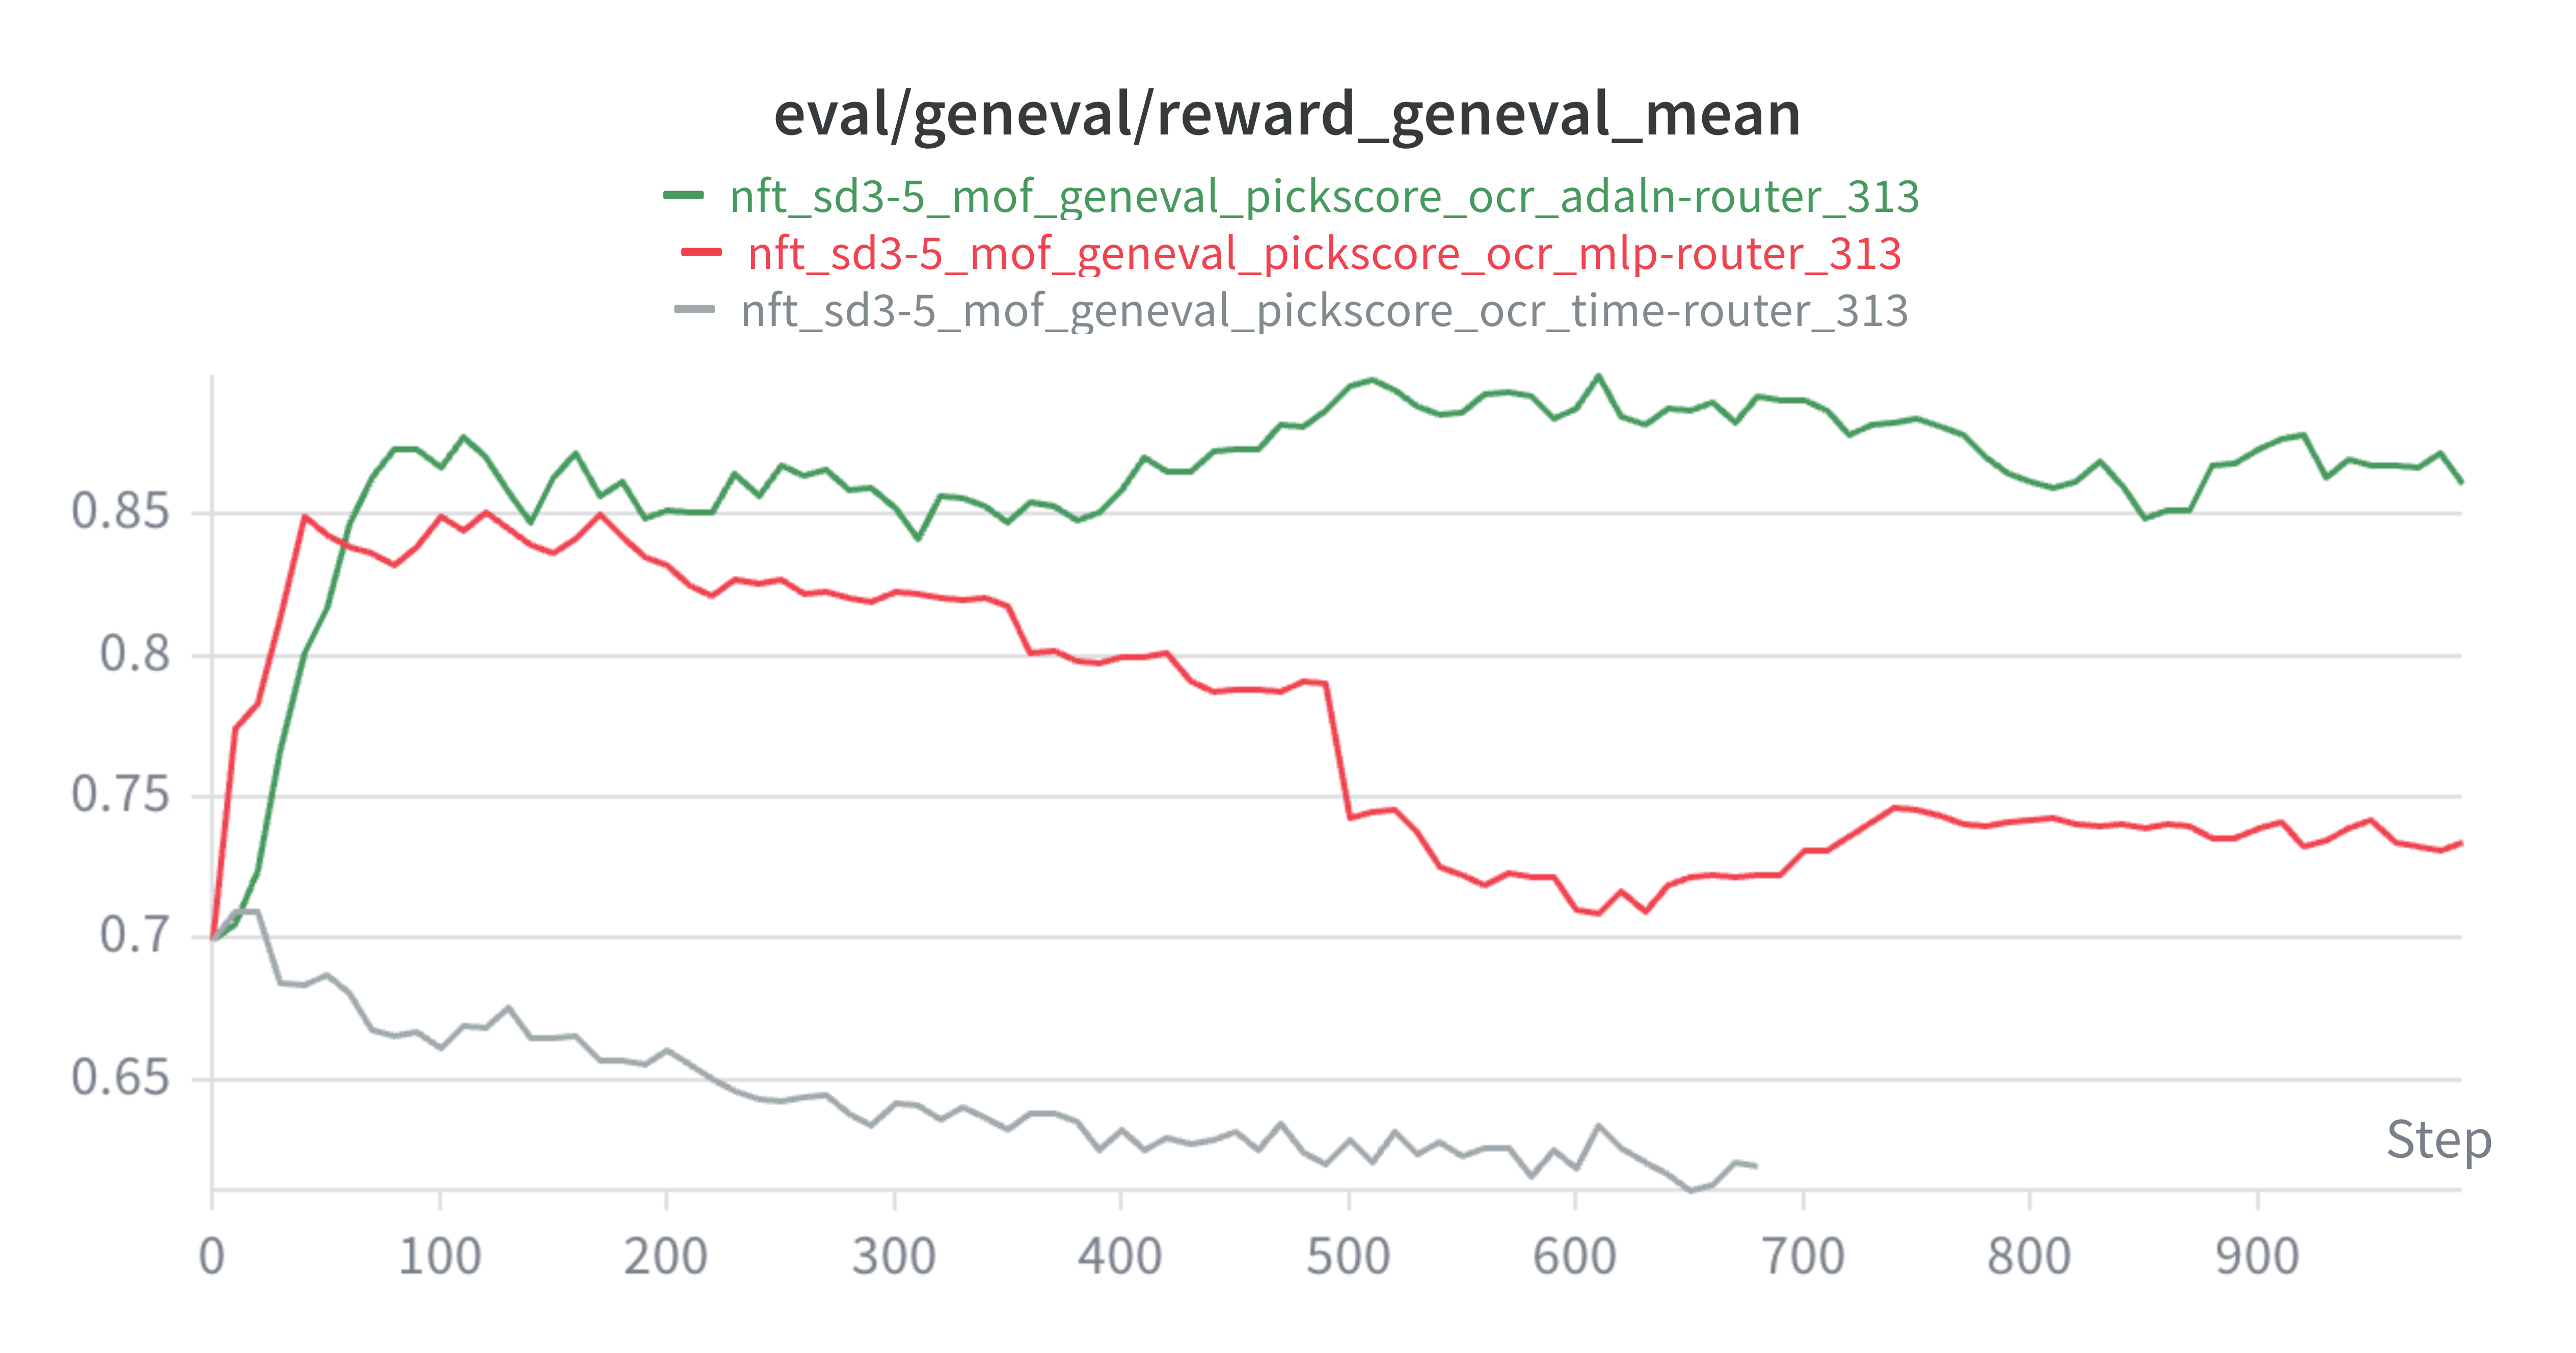
\includegraphics[width=\textwidth]{figures/o1-suboptimal-geneval.png}
\caption{GenEval eval reward}
\label{fig:o1_geneval}
\end{subfigure}\hfill
\begin{subfigure}{0.33\textwidth}
\centering
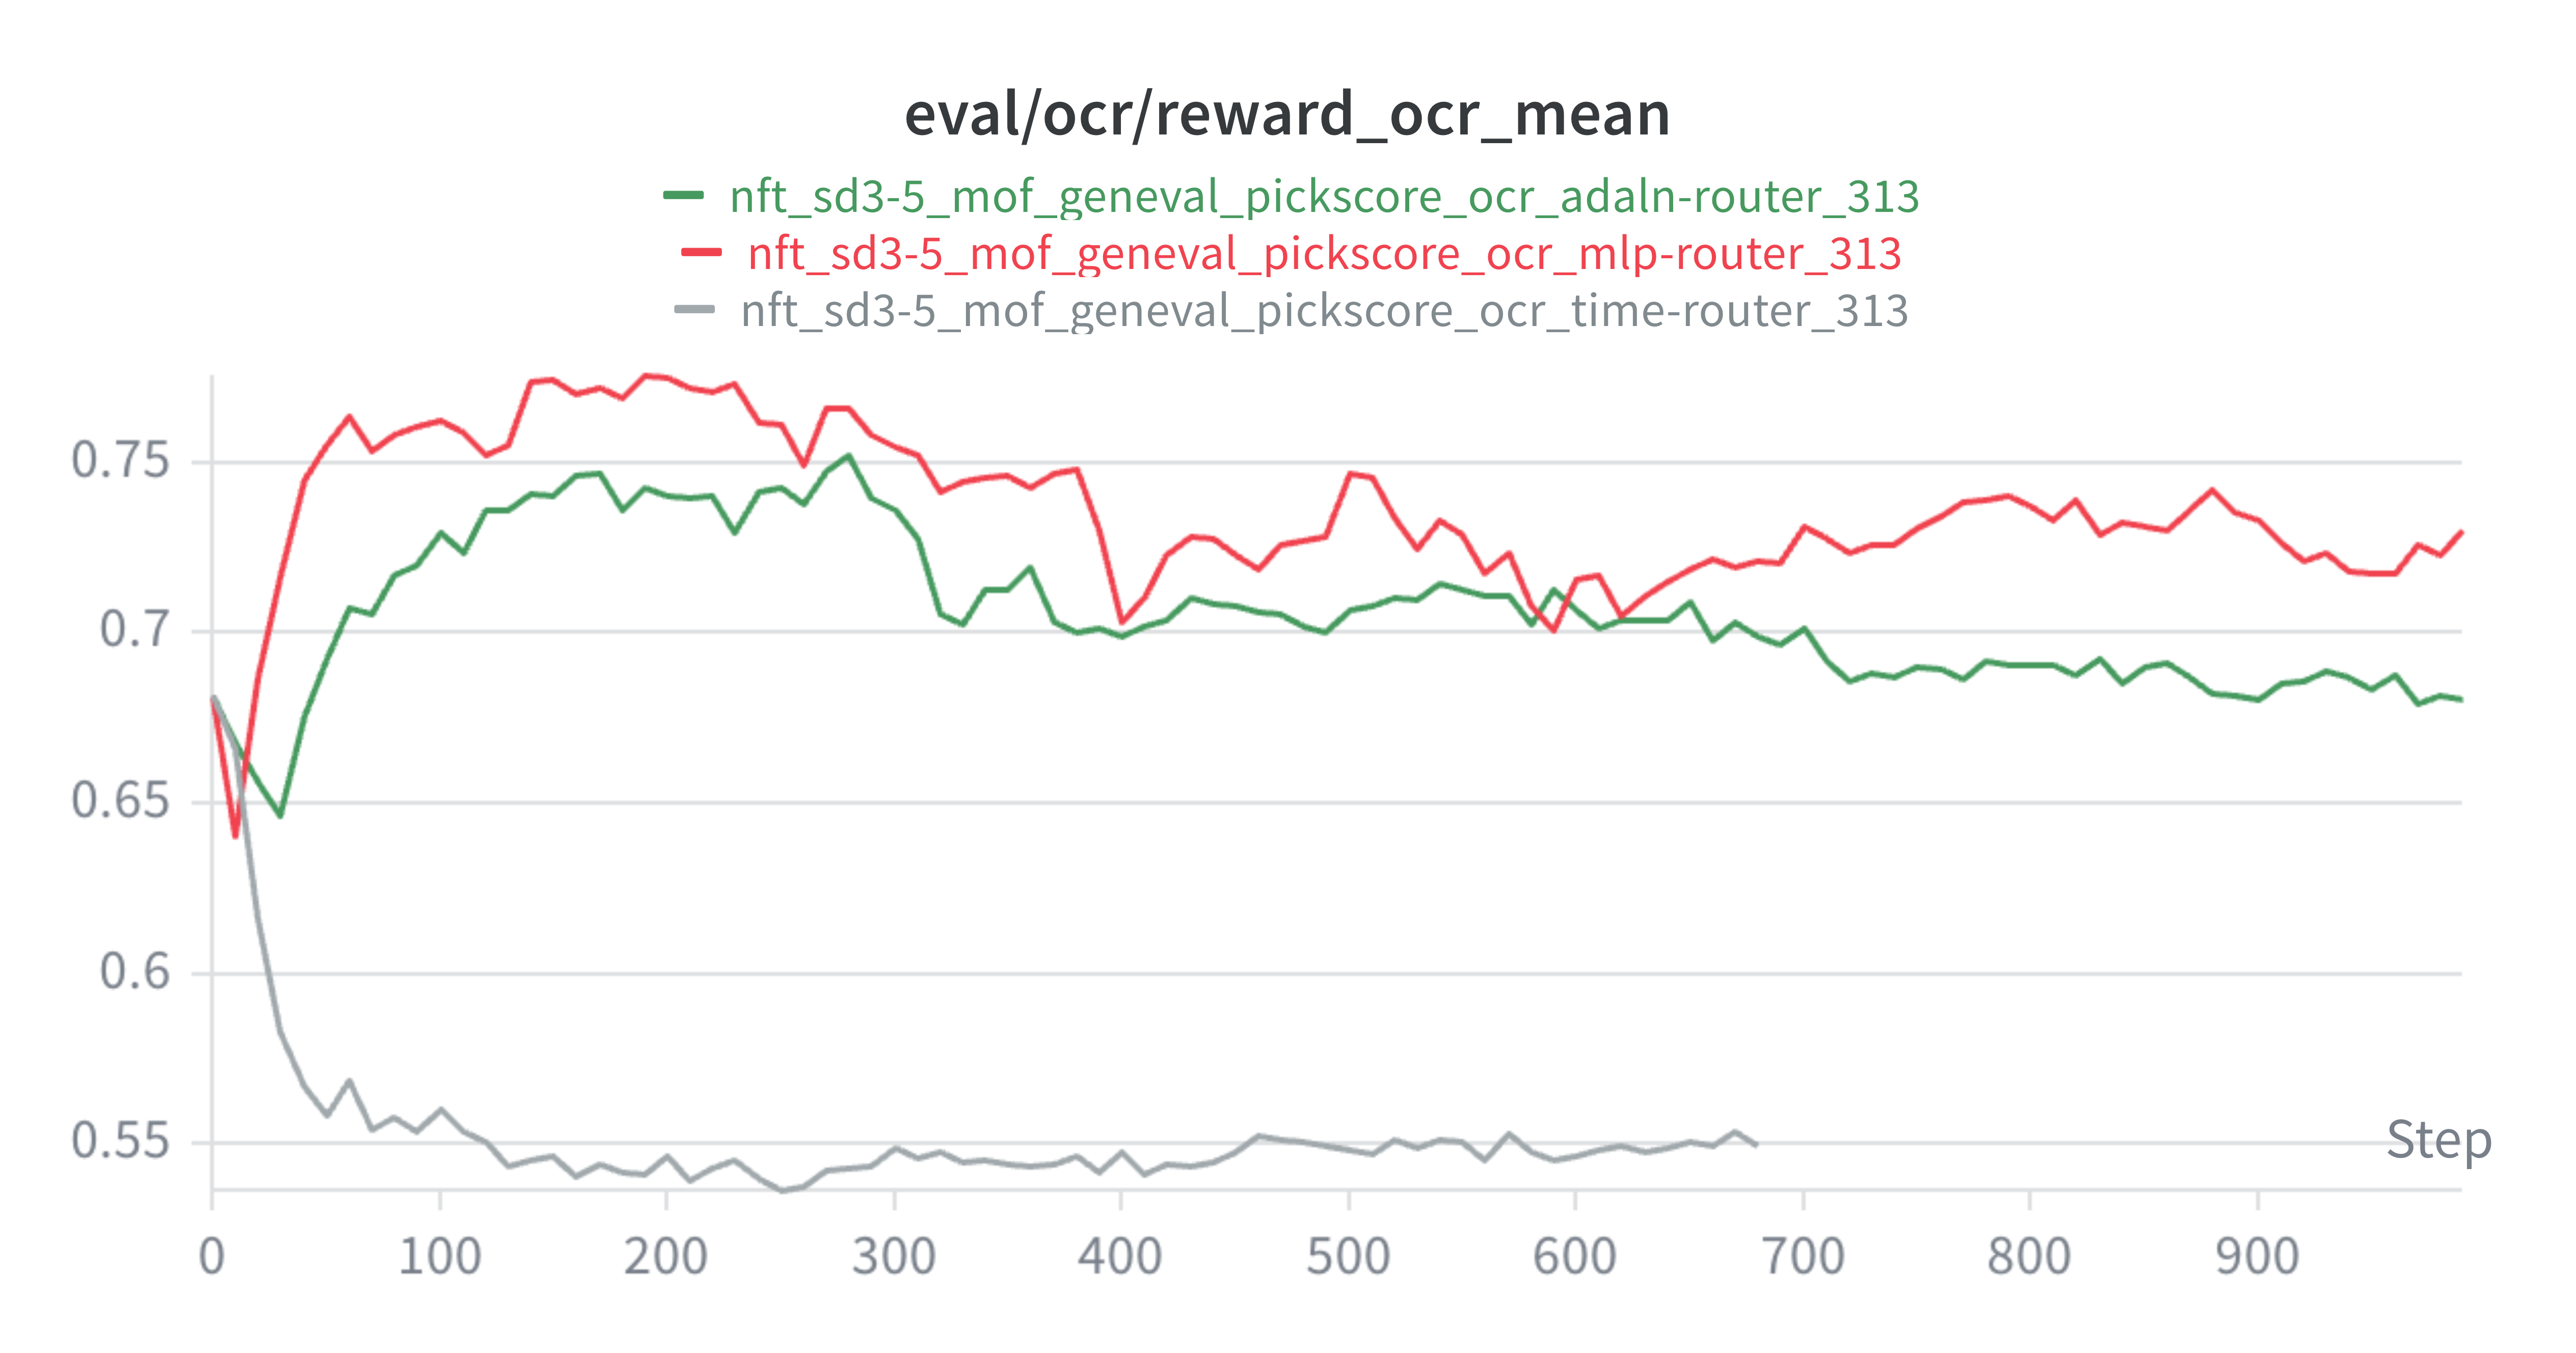
\includegraphics[width=\textwidth]{figures/o1-suboptimal-ocr.png}
\caption{OCR eval reward}
\label{fig:o1_ocr}
\end{subfigure}\hfill
\begin{subfigure}{0.33\textwidth}
\centering
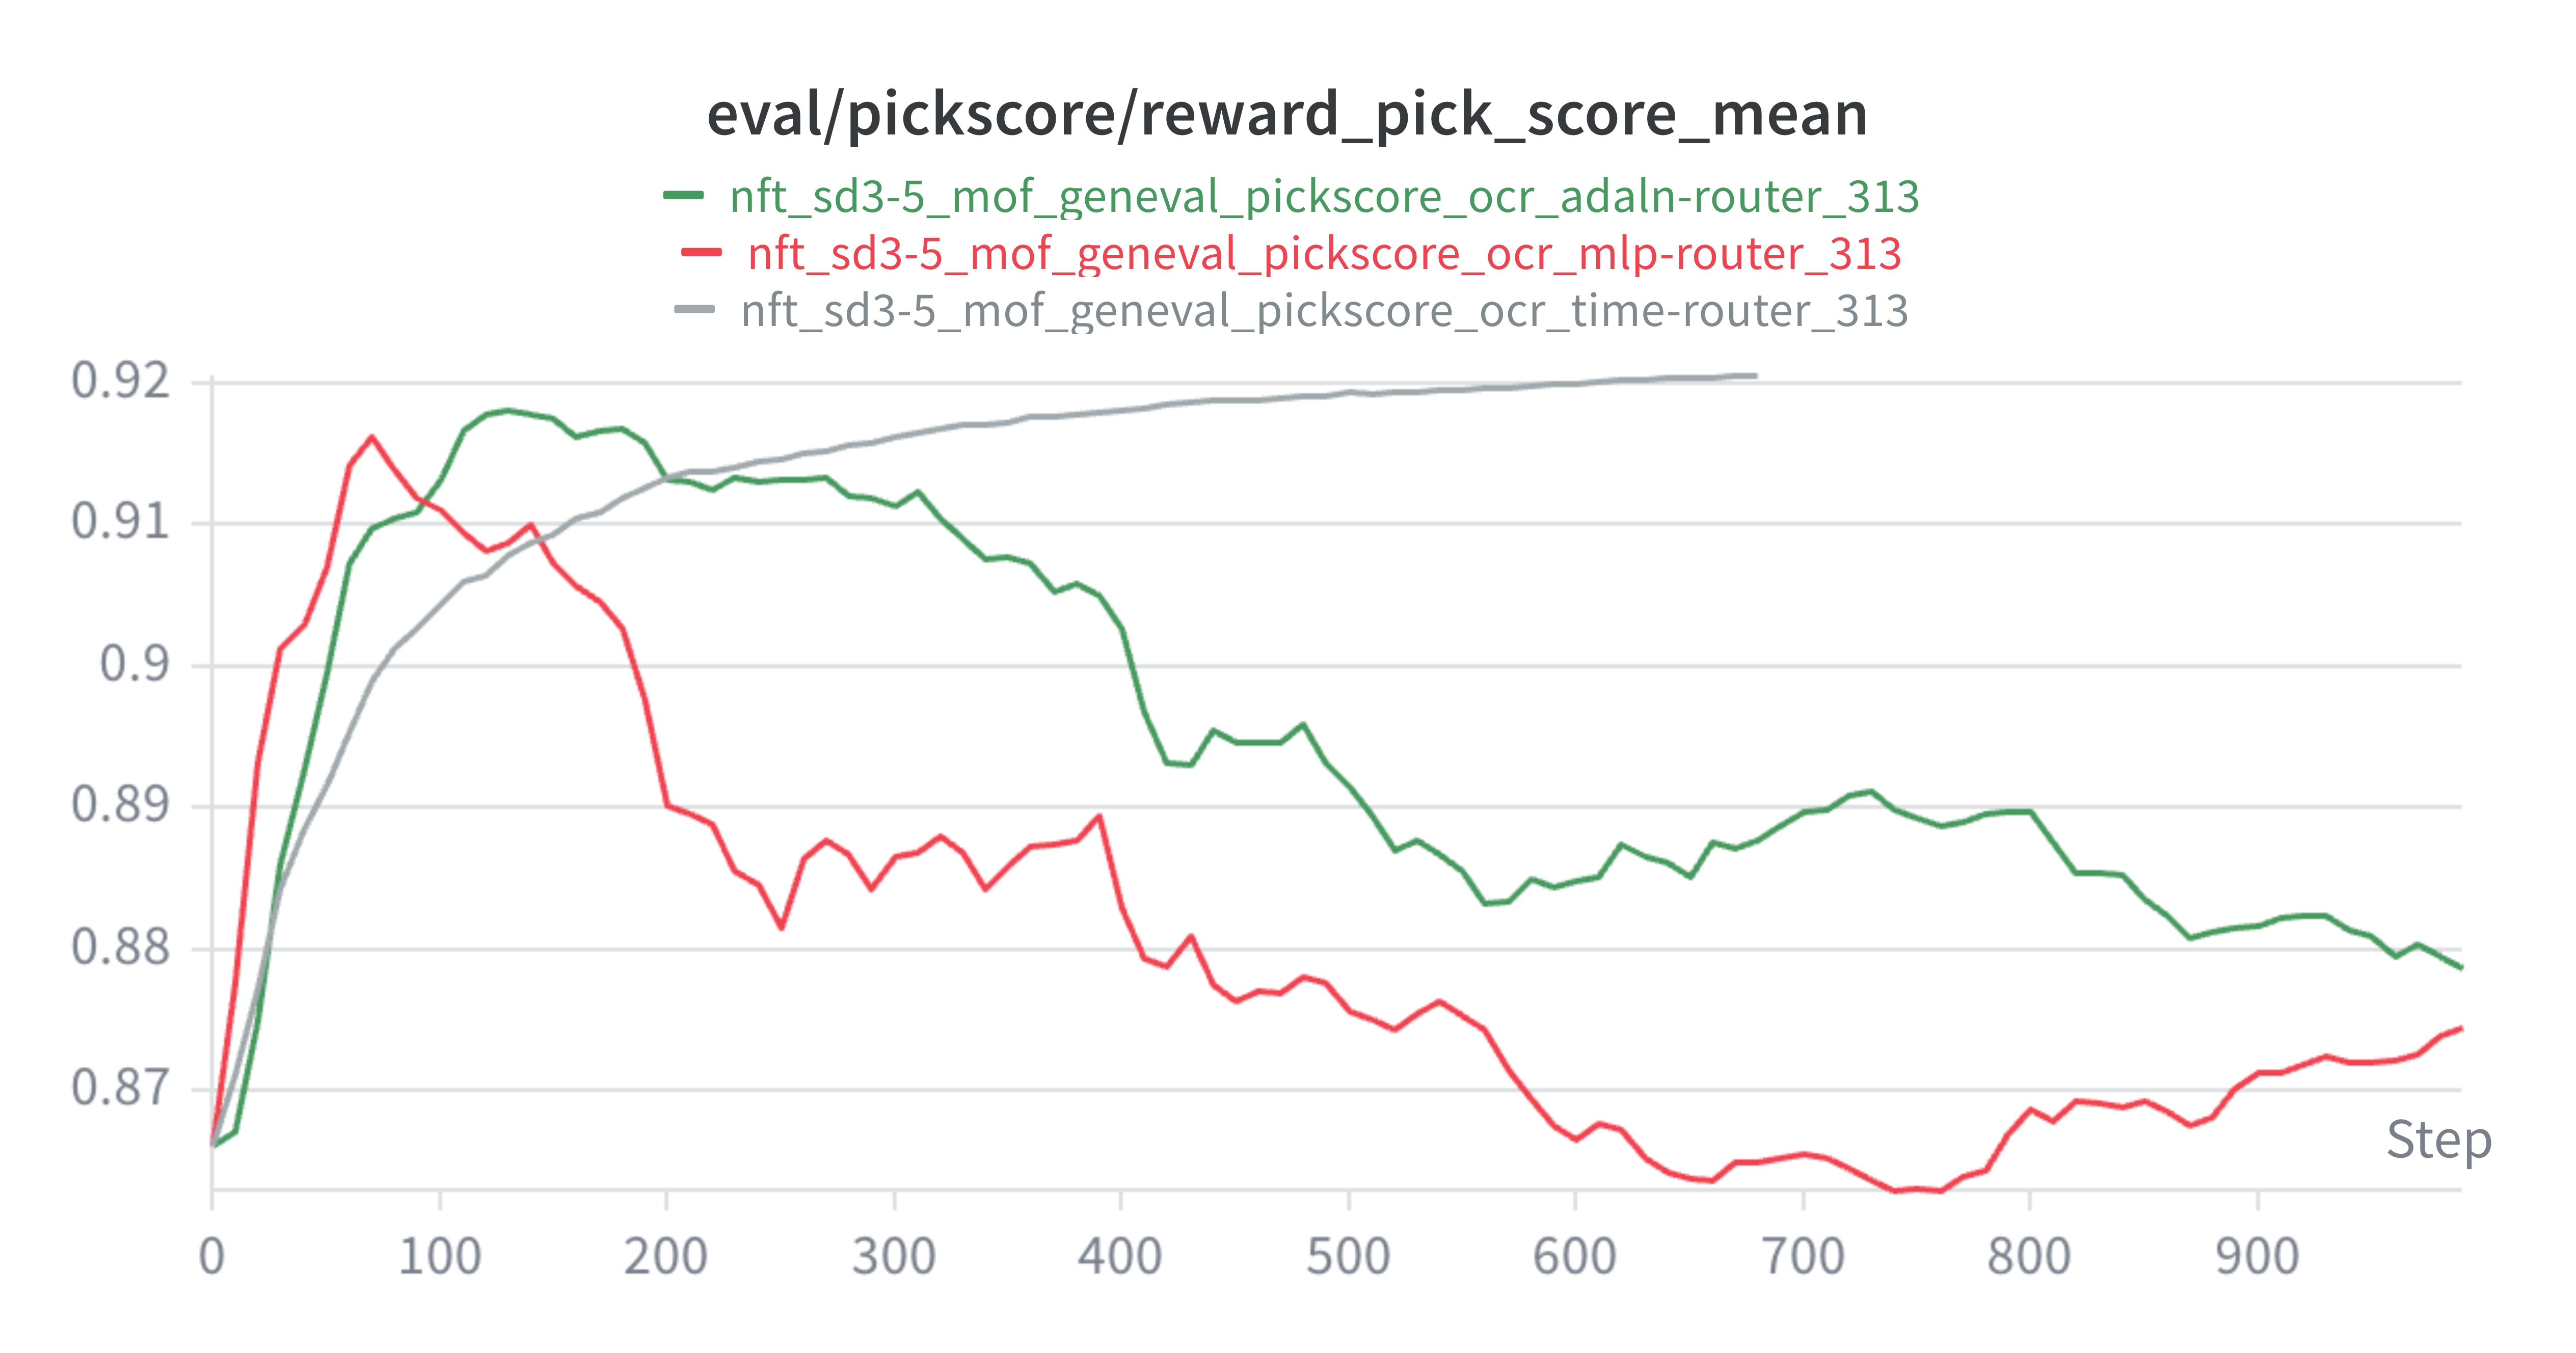
\includegraphics[width=\textwidth]{figures/o1-suboptimal-pickscore.png}
\caption{PickScore eval reward}
\label{fig:o1_pickscore}
\end{subfigure}
\caption{O1（用训练复合 reward 做 NFT）下三种神经 router 变体的 eval reward 曲线：
\textcolor{green!50!black}{adaLN-router（绿）}、\textcolor{red}{MLP-router（红）}、
\textcolor{gray}{Time-router（灰）}。没有任何一个变体能让三项 in-domain reward 同时维持
高位：\textcolor{gray}{Time-router} 把 universal 的 PickScore 单调推到最高
（\subref{fig:o1_pickscore}，$\sim0.92$），却让 OCR（\subref{fig:o1_ocr}，崩到 $\sim0.55$）
与 GenEval（\subref{fig:o1_geneval}，降到 $\sim0.62$）严重坍缩；\textcolor{green!50!black}{adaLN}
守住 GenEval（$\sim0.86$）但 OCR/PickScore 后期下滑；\textcolor{red}{MLP} 的 GenEval 后期
掉到 $\sim0.73$。即优化\emph{同一个}复合 reward 收敛到一个 trade-off——某项 in-domain
metric 必然退化，印证 O1 的``平凡 / 坍缩''结局。}
\label{fig:o1_suboptimal}
\end{figure}

\begin{remark}[O1 的根本局限]
\label{rem:o1}
O1 与造 teacher 用的是\emph{同一把尺子}$\{R_k\}$，因此``最好的混合 $=$ reward 最高的混合''
是同义反复。它暗示：在``旧 reward''指标上，可能\emph{不存在}显著优于平凡解的混合——平凡
解已逼近该指标的可达上界。要超越，必须换一把尺子或换一个目标空间。
\end{remark}

\subsection{O2：用一个更强的 reward 做 RL}
\label{ssec:o2}

\paragraph{定义.} 取 $Q_{\text{O2}}(v_\lambda)=\E_{p}[R^{\dagger}(\mathrm{ODE}(v_\lambda;p))]$，
其中 $R^\dagger$ 是比 $\{R_k\}$ 更强/更可靠的 reward（如更强 VLM judge）。

\paragraph{元问题.} O2 立刻引出两个必须回答的对照问题：
\begin{enumerate}[leftmargin=1.5em]
\item 若有更强的 $R^\dagger$，为何不\emph{直接}用 $R^\dagger$ 对 base 做 RL？
\item ``先 RL（造 teacher）再 OPD 混合''相比``直接 multi-reward RL''或``分阶段 RL''
究竟好在哪？（这正是 \texttt{mof\_vs\_direct\_opd\_gap.tex} 的 A vs.\ B 对比所形式化的：
A 的 reward 上界不低于 B，但实得取决于 Stage-1 优化与蒸馏 gap。）
\end{enumerate}

\paragraph{reward false-negative.} O2 的动机部分来自 $\{R_k\}$ 的\emph{不可靠}：reward 会
产生 false-negative。例如一张\emph{背景美观、且含 GenEval 要求的正确物体与属性}的图像，
因背景干扰物体检测而被 GenEval 判低分（人眼判满分）；GenEval 偏好无背景图，PickScore 偏好
有背景图。混合模型有时能生成``人眼判定下 GenEval 正确且美观''的图像（人眼高分），却在
reward model 下是低分（图~\ref{fig:geneval_fn}）。

\begin{figure}[ht]
\centering
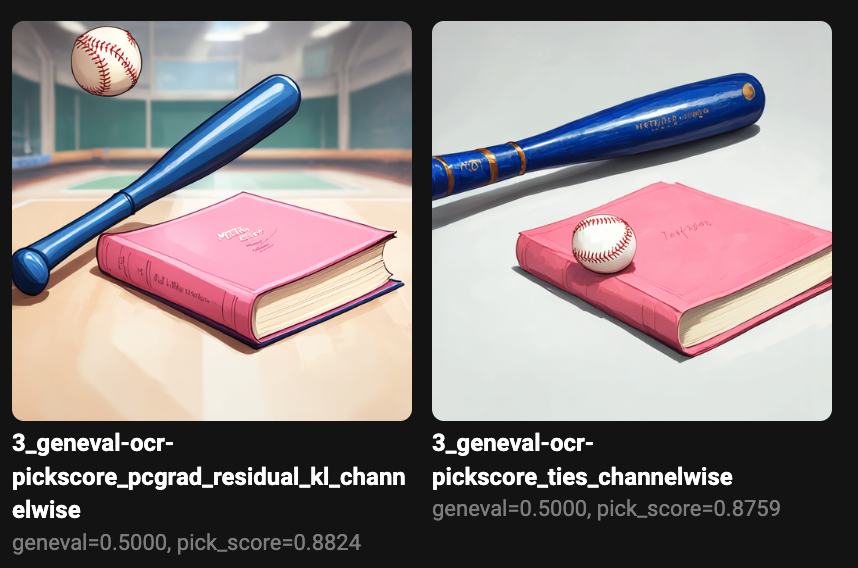
\includegraphics[width=0.5\textwidth]{figures/geneval-failed-case.png}
\caption{GenEval false-negative 实例。Prompt：\emph{``a photo of a blue baseball bat and a
pink book''}。两张生成图都\emph{清晰包含}蓝色棒球棒与粉色书本（人眼判定物体、颜色属性与
计数均正确，且构图美观），却均被 GenEval 判为 $0.5$.}
\label{fig:geneval_fn}
\end{figure}

\subsection{O3：training-free user study / 成对偏好}
\label{ssec:o3}

\paragraph{定义.} 不用 reward；对若干候选混合方案在同一 prompt 上离线生成图像
（图~\ref{fig:offline_comp}），用 user study / pairwise preference 直接比较，选出最优混合后
再蒸馏到单模型。形式上 $Q_{\text{O3}}=$ 人类偏好胜率。

\paragraph{分析.} 优点：\emph{training-free}，且以人眼为 ground truth，天然规避 reward
false-negative 与自循环；确定最优混合后只需一次蒸馏。

\begin{figure}[ht]
\centering

\includegraphics[width=\textwidth]{figures/offline-comparison.png}
\caption{O3 的离线对比示例（prompt：\emph{``a photo of a blue baseball bat and a pink
book''}）。}
\label{fig:offline_comp}
\end{figure}

\subsection{O4：最小化与 pretrained 模型的 KL}
\label{ssec:o4}

\paragraph{定义.}
\begin{equation}
\begin{aligned}
Q_{\text{O4}}(v_\lambda)
&= \underbrace{-\,\E_{(x_t,t)\sim q_\lambda}\!\big[\KL\big(p_\lambda(\cdot\mid x_t)\,\|\,
p_{\base}(\cdot\mid x_t)\big)\big]}_{=\,-\,\E[\,w_t\|v_\lambda-v_{\base}\|^2\,]}\\[2pt]
&\quad+\;\underbrace{\textcolor{red}{\;c_{\mathrm{ent}}\,\E_b\!\big[H(\lambda)\big]
\;-\;c_{\mathrm{unif}}\,\E_b\!\big[\,\big\|\lambda-\tfrac{1}{K}\mathbf{1}\big\|^2\,\big]\;}}
_{\text{（optional balancing terms default 0, i.e. pure KL-to-base）}} .
\end{aligned}
\label{eq:o4}
\end{equation}
含义：在\emph{最小化 distribution shift}的前提下，获取部分 multi-teacher 的 performance
gain——第一项惩罚 $\|v_\lambda-v_{\base}\|$，把 student 约束在 base 附近，从而抑制对各 teacher
hacking 成分的过度叠加。其余\textcolor{red}{两项为\emph{可选}平衡项}（默认系数 $0$）：
\begin{itemize}[leftmargin=1.5em]
\item \textbf{entropy bonus} $c_{\mathrm{ent}}\,\E_b[H(\lambda)]$：以路由权重的熵作奖励，
$c_{\mathrm{ent}}>0$ 让权重保持\emph{分散}、避免坍缩到单一 teacher（仅 softmax 参数化适用）；
对应配置项 \texttt{klmin\_entropy\_coeff}。
\item \textbf{uniform anchor} $-\,c_{\mathrm{unif}}\,\E_b\|\lambda-\tfrac{1}{K}\mathbf{1}\|^2$：
以到均匀分布 $1/K$ 的距离作惩罚，$c_{\mathrm{unif}}>0$ 把权重\emph{拉向均匀}；对应配置项
\texttt{klmin\_uniform\_anchor\_coeff}。
\end{itemize}
二者都在``贴近 base''与``保留多-teacher 混合''之间提供调节旋钮（$\E_b$ 为 batch 内对
per-sample 权重向量 $\lambda$ 取平均）。

\paragraph{现状.} 正在实验：目前在pure-KL-to-base下得到一个\emph{指标略高于 pretrained、图像质量与 pretrained相近}的模型。
这符合``适当微调''的直觉，但指标并不亮眼——因为它更接近未 RL-tuned 的 base，
在多个 prompt set 上的 reward 都偏低。换言之 O4 牺牲了 in-domain 峰值换取了平滑与稳健。

\subsection{O5：小规模真实数据 SFT}
\label{ssec:o5}

\paragraph{定义.} 收集一个小的\emph{真实图像}数据集，对混合模型（或其蒸馏 student）做 SFT，
即最小化留出真实数据上的 flow-matching 残差（对应
\texttt{mof\_mixing\_quality\_analysis.tex} 度量 A 的 $\mathrm{FMres}$ 作为 ground truth）。

\paragraph{分析.} 以\emph{真实数据分布}而非 reward 代理为 ground truth，因果上独立于
$\{R_k\}$，可同时抑制 hacking 与坍缩。尚未尝试（需收集真实数据）。必须比较的 baseline 是
\emph{直接在 base model 上 SFT}——若混合 $+$ SFT 不优于 base $+$ SFT，则混合这一步的价值
存疑。此外，sft的数据与base model的预训练数据分布存在偏差，这可能存在一些问题。

\subsection{五条目标对比}
\label{ssec:compare}

\begin{center}
\renewcommand{\arraystretch}{1.45}
\footnotesize
\begin{tabular}{@{}p{2.4cm}cccp{3.6cm}p{2.6cm}@{}}
\toprule
\textbf{目标 $Q$} & \textbf{需 reward?} & \textbf{prompt-dep.?} & \textbf{training-free?}
& \textbf{预期结果} & \textbf{对应 doc} \\
\midrule
O1 旧 reward RL & 是（旧 $\{R_k\}$） & 是（router） & 否 &
平凡解 / 坍缩，鱼与熊掌不可兼得 & ood\_guarantee, notes \\
O2 强 reward RL & 是（强 $R^\dagger$） & 是 & 否 &
元问题（vs 直接/分阶段 RL）；受 false-negative 制约 & vs\_direct\_opd\_gap, mixing\_quality \\
O3 user study & 否（人评） & \ding{55} 弱 & \ding{51} &
全局/粗粒度最优混合，难学 prompt-dependent & mixing\_quality \\
O4 min-KL-to-base & 否 & 是 & 否 &
接近 base、质量稳健、指标偏低（实验中） & 本文（新） \\
O5 真实数据 SFT & 否（需数据） & 是 & 否 &
取决于数据；baseline=base$+$SFT（未试） & mixing\_quality（度量 A） \\
\bottomrule
\end{tabular}
\end{center}

%% ============================================================
\section{综合与开放问题}
\label{sec:synthesis}
%% ============================================================

\subsection{统一视角：凸包内的约束微调}

本文把``合并 $K$ 个 teacher''重述为：先用凸组合 \eqref{eq:param} 把搜索空间约束在
multi-teacher 凸包内（保证合法 flow model 且参数极少），再用 \eqref{eq:framework} 在该
凸包内按某个目标 $Q$ 微调路由。DiffusionOPD 是 $Q=-\loss_{\OPD}$ 的特例，其解是凸包的
平凡点；O1--O5 则是对 $Q$ 的不同选择。\textbf{真正的开放问题不是如何优化，而是如何定义
$Q$（即``更好''）。}

\begin{tcolorbox}[colback=yellow!5,colframe=yellow!60!black,title=\textbf{核心论断}]
\begin{enumerate}[leftmargin=1.5em]
\item DiffusionOPD 最优 $=$ 平凡路由：单 teacher one-hot，多 teacher 监督权重均值
（命题~\ref{prop:trivial}、\ref{prop:multi}）；最优系数等于监督权重 $\pi_{k\mid s}$、
与 $(x_t,t)$ 无关。
\item 平凡解继承 single-reward teacher 的 hacking，在 in-domain 上坍缩/锐化
（定义~\ref{def:collapse}），需用独立于 reward、以真实数据为 ground truth 的判据
（precision--recall）才能诊断。
\item 由于混合本身是合法 flow model，``更好''$=$ 凸包约束下某目标 $Q$ 的最优；但在
\emph{旧 reward} 这把尺子下（O1），平凡解可能已近上界——``更高分 $\neq$ 更好''。
\item 因此有价值的方向是\emph{换尺子或换目标空间}：强 reward 但需打破自循环（O2）、
人评（O3）、最小 distribution shift（O4）、真实数据 ground truth（O5）。
\end{enumerate}
\end{tcolorbox}

\subsection{开放问题}
\begin{enumerate}[leftmargin=1.5em]
\item \textbf{``更好''的可操作定义}：能否给出一个\emph{因果上独立于训练 reward}、且可
\emph{prompt-dependent} 学习的标量 $Q$？（O3 独立但不 prompt-dependent；O1 prompt-dependent
但自循环。）
\item \textbf{O2 的对照}：在统一 setting 下实测``RL$\to$OPD混合'' vs.\ ``直接强-reward RL''
vs.\ ``分阶段 RL''，验证 \texttt{mof\_vs\_direct\_opd\_gap.tex} 的 A$\gtreqless$B 边界条件。
\item \textbf{O4 的价值}：简单来看O4的策略可能会比较有价值——其符合``适当微调''的直觉，但其指标上的劣势是否可以接受？
\item \textbf{其他“好”的定义？}是否存在其他好的定义？
\end{enumerate}

%% ============================================================
\section{与现有文档的关系}
\label{sec:relation}
%% ============================================================

本文是 roadmap / position 文档，承上启下地把姊妹文档串成一条线：

\begin{center}
\renewcommand{\arraystretch}{1.4}
\footnotesize
\begin{tabular}{@{}p{5.2cm}p{8.3cm}@{}}
\toprule
\textbf{文档} & \textbf{关系} \\
\midrule
\texttt{mof\_notes.tex} &
凸组合合法性、两阶段流水线、teacher 训练与保守 checkpoint 选择——其 affine-closure 与本文
附录~\ref{app:validity} 的自包含证明一致；\S\ref{ssec:hacking} 引其 teacher-training 经验。 \\
\texttt{mof\_vs\_direct\_opd\_gap.tex} &
MoF$\to$Distill (A) vs.\ route-by-source OPD (B) 的形式化；本文 \S\ref{ssec:trivial} 的
$\mathcal{T}_B\subsetneq\mathcal{T}_A$ 与 \S\ref{ssec:o2} 的元问题直接复用。 \\
\texttt{mof\_ood\_guarantee\_analysis.tex} &
OOD 严格超越的负面定理与不对称性；本文 \S\ref{ssec:o1}（O1 平凡 / 鱼与熊掌）的理论根据。 \\
\texttt{mof\_mixing\_quality\_analysis.tex} &
PoE/responsibility-weighted 真传输（其结论与本文附录~\ref{app:validity} 一致）、reward
自循环、reward-free 度量（FMres、precision--recall 等）——\S\ref{sec:pathology} 复用其
precision--recall，\S\ref{ssec:o3}--\ref{ssec:o5} 复用 FMres / 独立裁判。 \\
\texttt{mof\_per\_set\_analysis.tex} &
per-set Level-1 构造性保证与梯度分析；本文 \S\ref{ssec:goal} 目标层次的来源。 \\
\texttt{mof\_reward\_design.tex} &
复合 reward 与 advantage 设计；本文 \S\ref{ssec:o1} 复合目标 $F^{(s)}$ 的定义对齐。 \\
\bottomrule
\end{tabular}
\end{center}

\paragraph{参考.} DiffusionOPD: \emph{A Unified Perspective of On-Policy Distillation in
Diffusion Models}（Li et al., 2026），\url{https://github.com/ali-vilab/DiffusionOPD}。

%% ============================================================
\appendix
\section{凸组合的合法性：仿射闭包、真传输与 well-posedness}
\label{app:validity}
%% ============================================================

本附录给出 \S\ref{ssec:param} 所用结论的\emph{自包含}推导。记 marginal density $p_t(x)$
与速度场 $v(x,t)$ 满足连续性方程
\begin{equation}
\partial_t p_t + \nabla\!\cdot\!\big(p_t\,v\big)=0 .
\label{eq:continuity}
\end{equation}

\subsection{共享 marginal 下的仿射闭包}
\label{ssec:app_closure}

\begin{proposition}[仿射闭包]
\label{prop:app_closure}
设 $v^{(1)},\dots,v^{(K)}$ 传输\emph{同一} marginal path $p_t$，即各自满足
\eqref{eq:continuity}。则对任意 $\lambda\in\R^K$ 且 $\sum_k\lambda_k=1$（允许 $\lambda_k<0$
或 $>1$），仿射组合 $v_\lambda=\sum_k\lambda_k v^{(k)}$ 也满足 \eqref{eq:continuity}（对同一
$p_t$）。
\end{proposition}

\begin{proof}
由 $\nabla\!\cdot$ 的线性性，
\begin{align*}
\partial_t p_t+\nabla\!\cdot\!\big(p_t v_\lambda\big)
&=\partial_t p_t+\sum_k\lambda_k\,\nabla\!\cdot\!\big(p_t v^{(k)}\big)\\
&=\sum_k\lambda_k\underbrace{\big[\partial_t p_t+\nabla\!\cdot\!(p_t v^{(k)})\big]}_{=\,0}
+\Big(1-\textstyle\sum_k\lambda_k\Big)\partial_t p_t
=\Big(1-\textstyle\sum_k\lambda_k\Big)\partial_t p_t .
\end{align*}
对非定常（time-varying）$p_t$，末项为零当且仅当 $\sum_k\lambda_k=1$。
\end{proof}

\begin{remark}[仿射即可，凸性非必需]
\label{rem:app_affine}
证明只用到 sum-to-one，\emph{未}用 $\lambda_k\ge0$，故权重可为负或超过 $1$——classifier-free
guidance $v=(1-w)v_{\text{uncond}}+w\,v_{\text{cond}}$（$w>1$）即典型的非凸仿射组合。反之，
若 $\sum_k\lambda_k=c\neq1$，残留项 $(1-c)\,\partial_t p_t$ 等价于把速度场整体缩放，是一次
时间重参数化，会把样本推离该 marginal path。
\end{remark}

\subsection{非共享 marginal：真传输是 responsibility-weighted}
\label{ssec:app_transport}

\begin{proposition}[混合 marginal 的真传输]
\label{prop:app_transport}
连续性方程关于\emph{对} $(p,\,m)$（其中 flux $m=p\,v$）是线性的。若各
$\big(p_t^{(k)},\,p_t^{(k)}v^{(k)}\big)$ 满足 \eqref{eq:continuity}，则混合 marginal
$p_t^{\mathrm{mix}}=\sum_k\lambda_k p_t^{(k)}$（$\lambda_k\ge0,\ \sum_k\lambda_k=1$）由
\begin{equation}
\tilde v_\lambda(x,t)=\frac{\sum_k\lambda_k\,p_t^{(k)}(x)\,v^{(k)}(x,t)}
{\sum_k\lambda_k\,p_t^{(k)}(x)}=\sum_k r_k(x,t)\,v^{(k)}(x,t),\qquad
r_k=\frac{\lambda_k p_t^{(k)}}{\sum_j\lambda_j p_t^{(j)}}
\label{eq:app_resp}
\end{equation}
传输（$\sum_k r_k=1$）。且 $\tilde v_\lambda=v_\lambda$ 当且仅当所有 $p_t^{(k)}$ 在该点相等
（此时 $r_k\equiv\lambda_k$）。
\end{proposition}

\begin{proof}
取 flux $m_t=\sum_k\lambda_k p_t^{(k)}v^{(k)}$，则
$\partial_t p_t^{\mathrm{mix}}+\nabla\!\cdot m_t
=\sum_k\lambda_k\big[\partial_t p_t^{(k)}+\nabla\!\cdot(p_t^{(k)}v^{(k)})\big]=0$，
故 $(p_t^{\mathrm{mix}},m_t)$ 满足 \eqref{eq:continuity}；传输 $p_t^{\mathrm{mix}}$ 的速度即
$m_t/p_t^{\mathrm{mix}}=\tilde v_\lambda$。
\end{proof}

\begin{remark}[这解释了为何命题~\ref{prop:app_closure} 必须共享 marginal]
\label{rem:app_why_shared}
常权平均 $v_\lambda=\sum_k\lambda_k v^{(k)}$ 与真传输 $\tilde v_\lambda$（responsibility 权）
\emph{仅}在所有 $p_t^{(k)}$ 重合时一致。teacher 经 RL/LoRA 微调后 marginal 被\emph{有意}
推移，彼此不同，故 $v_\lambda$ 一般\emph{不}传输 $p_t^{\mathrm{mix}}$，命题~\ref{prop:app_closure}
的精确性随之失效。
\end{remark}

\subsection{为何 MoF 不依赖上述合法性}
\label{ssec:app_wellposed}

\begin{remark}[well-posed ODE 已足够]
\label{rem:app_wellposed}
\leavevmode
\begin{enumerate}[leftmargin=1.5em]
\item 对任意足够正则的向量场，ODE $\dot x_t=v_\lambda(x_t,t)$ 解存在且唯一，把先验
pushforward 到\emph{某}分布 $\tilde p_t$——它一般既非 $p_t^{\mathrm{mix}}$、也非任一 teacher
marginal。
\item MoF 把 $v_\lambda$ \emph{直接}当采样器：rollout、计算 reward/advantage、或用作蒸馏
target，全部基于其\emph{实际}生成的样本，从不预设它传输某个指定 marginal。因此对 RL/LoRA
teacher 而言，命题~\ref{prop:app_closure} 的失效只否定``$v_\lambda$ 是某干净分布的合法
FM''这一\emph{解释}，并不影响 \S\ref{sec:convex} 之后的任何推导与流水线。
\item 近似的强弱沿时间不均匀：高噪声端各 marginal 同趋 $\N(0,I)$、近似最好，越靠近数据端
分歧累积、近似越差；在 one-hot 顶点（$\lambda=\bm e_k$，即 DiffusionOPD 平凡解）
$v_\lambda=v^{(k)}$ 严格合法，近似仅在 simplex 内部（真正混合）被调用。其定量误差界本文不作
声称。
\end{enumerate}
\end{remark}

\noindent 以上命题与 \texttt{mof\_notes.tex}、\texttt{mof\_mixing\_quality\_analysis.tex}
中相应结论一致，此处给出自包含证明，正文 \S\ref{ssec:param} 不再依赖外部文档。

\end{document}
